%
% Modo de operación CBC, capítulo de antecedentes.
% Proyecto Lovelace.
%

\subsubsection{\textit{Cipher-block Chaining} (CBC)}
\label{sec:cbc}

En \gls{gl:cbc} la salida del bloque uno se introduce (junto con
el siguiente bloque del mensaje) en el bloque dos, y así en sucesivo.
Para poder replicar este comportamiento en todos los bloque, este
\gls{gl:modo_de_operacion} necesita un argumento extra a la entrada: un
\gls{gl:vector_de_inicializacion}. De esta manera la salida del bloque $ i $
depende de todos los bloques anteriores; esto incrementa la seguridad con
respecto a \gls{gl:ecb}.

\begin{figure}
  \centering
  \begin{subfigure}{0.45\textwidth}
    \begin{center}
      \subimport{diagramas/}{modo_cbc.tikz.tex}
      \caption{Cifrado.}
    \end{center}
  \end{subfigure}
  \begin{subfigure}{0.45\textwidth}
    \begin{center}
      \subimport{diagramas/}{modo_cbc_inverso.tikz.tex}
      \caption{Descifrado.}
    \end{center}
  \end{subfigure}
  \caption{\Gls{gl:modo_de_operacion} \gls{gl:cbc}.}
  \label{figura:cbc}
\end{figure}

En la figura~\ref{figura:cbc} se muestran los diagramas esquemáticos para
cifrar y descifrar; en los pseudocódigos~\ref{cbc:1} y~\ref{cbc:2} se muestran
unos de los posibles algoritmos a seguir. Es importante notar que mientras que
el proceso de cifrado debe ser forzosamente secuencial (por la dependencias
entre salidas), el proceso de descifrado puede ser ejecutado en paralelo.

% Lástima que con los escapes en modo matemático dentro de los pseudocódigos
% se pierda totalmente la ventaja de trabajar con fuentes mono: por eso
% la alineación tan rara de los comentarios del próximo pseudocódigo.

\begin{pseudocodigo}[%
    caption={\Gls{gl:modo_de_operacion} \gls{gl:cbc}, cifrado.},
    label={cbc:1}%
  ]
    entrada: llave $ k $; vector de inicialización $ VI $;
             bloques de mensaje $ Bm_1, Bm_2 \dots Bm_n $.
    salida:  bloques de mensaje cifrado $ Bc_1, Bc_2 \dots Bc_n $.
    inicio
      $Bc_0$ $\gets$ $ VI $                        // El vector de inicialización
      para_todo $Bm$               // entra al primer bloque.
        $Bc_i$ $\gets$ E($k$, $Bm_i \oplus Bc_{i - 1}$)
      fin
      regresar $Bc$
    fin
\end{pseudocodigo}

\begin{pseudocodigo}[%
    caption={\Gls{gl:modo_de_operacion} \gls{gl:cbc}, descifrado.},
    label={cbc:2}%
  ]
    entrada: llave $ k $; vector de inicialización $ VI $;
             bloques de mensaje cifrado $ Bc_1, Bc_2 \dots Bc_n $.
    salida:  bloques de mensaje original $ Bm_1, Bm_2 \dots Bm_n $.
    inicio
      $Bc_0$ $\gets$ $ VI $
      para_todo $Bc$
        $Bm_i$ $\gets$ $D_k$($Bc_i$) $\oplus$ $Bc_{i-1}$
      fin
      regresar $Bm$
    fin
\end{pseudocodigo}

\subsection{CBC-MAC}
Este algoritmo está basado en el modo de operación \gls{gl:cbc} y una función
$F$ que puede ser, por ejemplo, un cifrado por bloques. Se encarga de
cifrar con una llave $l_1$ todo el mensaje $m$, pero lo único que se toma en
cuenta es el último bloque, que es tomado como el código de autenticación
(véase figura~\ref{mac:cbc1}). En algunos casos, se cifra de nuevo, con la misma
función $F$, pero utilizando una llave $l_2$ distinta (véase
figura~\ref{mac:cbc2}).
% 
% CBC-MAC es considerado seguro cuando el mensaje $m$ tiene una longitud
% múltiplo del tamaño de bloque del cifrado por bloques. Como se le han
% encontrado varias vulnerabilidades, algoritmos basados en CBC-MAC han sido
% propuestos, tales como el \textit{eXtended CBC} o el \gls{gl:omac}.
%
% \begin{figure}
%   \begin{center}
%     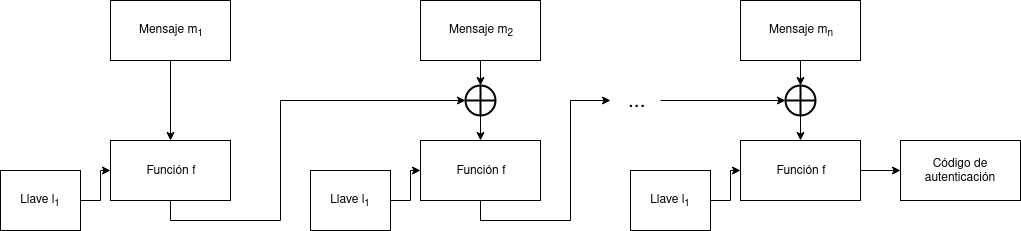
\includegraphics[width=0.9\linewidth]{diagramas/cbcmac.png}
%     \caption{Esquema de CBC-MAC simple.}
%     \label{mac:cbc1}
%   \end{center}
% \end{figure}
%
% \begin{figure}
%   \begin{center}
%     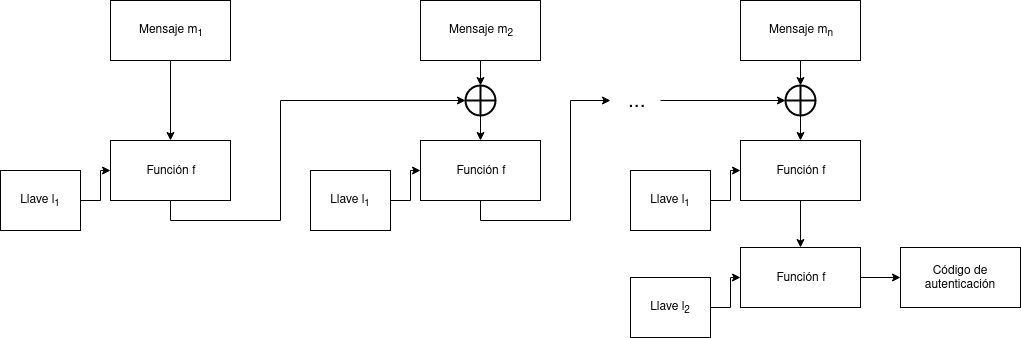
\includegraphics[width=0.9\linewidth]{diagramas/cbcmaclb.png}
%     \caption{Esquema de CBC-MAC con el último bloque cifrado.}
%     \label{mac:cbc2}
%   \end{center}
% \end{figure}
